\chapter{Concursos}
\label{ch:concursos}

Existen diferentes tipos de concurso o situaciones en las que puedes
necesitar resolver un problema en un breve espacio de tiempo, una de
las cosas más interesantes de los concursos es que el problema suele
estar escondido en la literatura del enunciado, es decir, no se
plantea directamente el problema a resolver, sino que se plantea una
situación real o no, esta situación conlleva la necesidad de realizar
una tarea de manera automática o calcular algunos resultados de dicha
situación. En este capítulo se presentan diferentes concursos. Todos
ellos acaban consistiendo en resolver una serie de problemas
matemáticos, algorítmicos, de grafos, etc. Los concursos pueden tener
diferentes características o normas, como por ejemplo, pueden ser
presenciales u online, por equipos o individuales, con acceso a
internet o sin él, jueces automáticos o humanos, los lenguajes de
programación permitidos etc.
\section{Online}
\label{sec:concursos:online}
Muchas de las grandes compañías de Internet, tienen concursos de
programación donde plantean una serie de retos de diferente
índole. Por ejemplo el ``Code Jam'' (Google) y el ``Tuenti’s Contest''
(Tuenti).\\

El primero tiene varias fases online que desembocan en una fase
presencial, tal y como puede apreciarse en la
Figura~\ref{fig:codejam}.\\

\begin{figure}[h]
\hrule\smallskip
\begin{center}
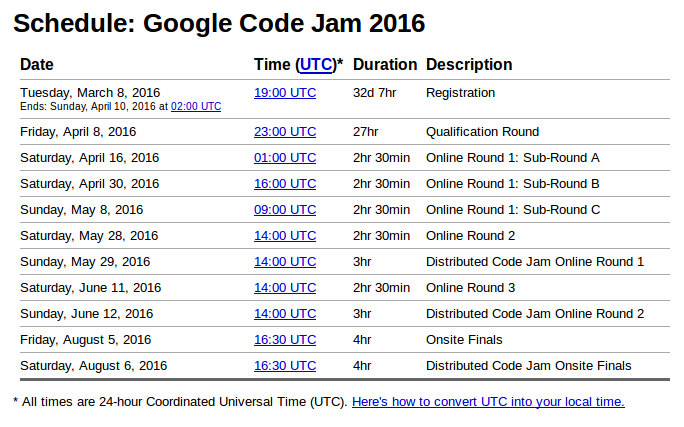
\includegraphics[width=1\textwidth]{fig/codejam.png}
\end{center}
\caption{Planificación del Code Jam Google 2016}
\label{fig:codejam}
\hrule
\end{figure}

El segundo concurso mencionado, ``Tuenti's Contest'', se realiza en
varios días de manera ininterrumpida. En este concurso no importa
tanto y el tiempo que tardas en resolver un problema sino la calidad
con que lo haces, dado que los problemas son revisados por jueces
reales y lo que buscan es la solución perfecta o idónea ya que el fin
último de este Concurso es la captación de programadores brillantes
que estén interesados en trabajar en Tuenti. Por eso, a los primeros
puestos se les ofrece una entrevista especial la que verifican que los
problemas entregados de manera online han sido realizados realmente
por ellos y se les ofrece un buen puesto de trabajo.
\\

En la categoría online encontramos también otra serie de concursos
como pueden ser ``las 12 uvas'', dónde el objetivo es resolver 12
problemas sencillos en el último día del año. Este concurso es
organizado por los hermanos Marco Antonio y Pedro Pablo Gómez, en este
año es patrocinado por Coritel.
\\

Como podemos observar, en los concursos online suelen ser de manera
individual y siempre acaba habiendo una comprobación de que el
participante es el autor de las soluciones entregadas.

\section{Presenciales}
\label{sec:concursos:presenciales}

En el caso de los concursos presenciales no hace falta una
comprobación dado que los problemas se resuelven bajo la supervisión y
unos jueces o colaboradores de estos. La principal dificultad en estos
concursos suele recaer en la organización del equipo, ya que, lo
normal, es disponer de un solo ordenador para todos los integrantes.\\

Un concurso de esta categoría puede ser ``ProgramaMe'', Organizado para
estudiantes de módulo superior e institutos y tiene lugar en la
Facultad de Informática de la Complutense. Los equipos están formados
tres personas.\\

Otro concurso, también organizado en la Facultad de Informática, es el
``Ada-Byron'' con motivo de la celebración de la semana de la
Informática se invita a los estudiantes de grado a participar. La
metodología es similar a ``ProgramaMe'' pero con un nivel de dificultad
mayor.\\

Estos concursos están inspirados en la SWERC (SouthWestern Europe
Regional Contest) que tiene nivel europeo, donde alrededor de 50
equipos compiten por conseguir una plaza en el concurso ``ACM
International Collegiate Programming Contest'' que tiene carácter
mundial. En este concurso, los equipos también están formados por tres
integrantes y una buena organización del equipo puede ser la clave del
éxito. Los problemas tienen mayor dificultad y requieren habitualmente
conocimientos previos y experiencia en la resolución de ese tipo de
problemas. La clasificación se realiza en primer lugar por número de
problemas resueltos y en caso de empate por el tiempo requerido para
hacerlo, teniendo en cuenta que realizar un envío de una solución
errónea se penalizará con la suma de 20 minutos. Es por esto que no
solo es importante saber programar, sino hacerlo rápido, bien y
aprendiendo a testear el código en especial para los casos límite.

\subsection{Organización del Equipo}
\label{sec:concursos:organizacion}

Como ya he comentado, la organización suele ser crucial a la hora de
resultar productivo. Sea cual sea tu organización debes guiarte por
cinco ideas básicas:

\begin{enumerate}
\item Saber programar sobre papel. Con un solo ordenador, lo normal es
  que otro miembro del equipo esté programando y no puedas
  interrumpirlo en ese momento.

\item Analizar y preparar casos de test extremos. Lo mejor es meter
  estos casos en un archivo que posteriormente se redirija como
  entrada al programa, esto evitará perder mucho tiempo y errores
  innecesarios.

\item Programar en un IDE y compilar en consola. Los IDE por lo
  general te ayudan a autocompletar código o a encontrar errores
  sintácticos mientras programas, por eso es bueno que todo el equipo
  use uno y a ser posible el mismo. Sin embargo, la consola es nuestra
  amiga a la hora de compilar y ejecutar el código dado que nos ofrece
  mayor flexibilidad a la hora de ejecutar con texto de entrada
  predeterminado o improvisar soluciones. Además el juez automático
  compilará en una consola y no auto-incluirá librerías tal y como
  hacen algunos IDEs.

\item Enviar e Imprimir. Normalmente se permite imprimir código por lo
  que una buena práctica al subir una solución es mandarla imprimir y
  dejar a otro sentarse a programar el siguiente problema, de esta
  manera si te has equivocado en tu respuesta tendras en papel el
  código y podrás analizarlo sin perder tiempo de teclado.

\item Tener buena relación con los integrantes del equipo. La
  confianza en tus compañeros y conocer los puntos fuertes y débiles
  de cada uno programando ayuda a hacer más fuerte el equipo.
\end{enumerate}
Viendo estos consejos se puede apreciar que lo más importante es no
perder tiempo de teclado. De ahí que sea necesaria una organización
previa y que todo el equipo la conozca.\\

Aún así existen diferentes formas de organizarse, casi tantas como
equipos existen, por ello a continuación ilustro un par de
posibilidades:
\begin{itemize}
\item El escritor. Si en el equipo hay alguien que puede escribir un
  código a gran velocidad sin errores, aunque no necesariamente haya
  pensado él la solución suele estar a cargo todo el tiempo del
  teclado. El concurso lo comenzará escribiendo un código plantilla
  donde incluirá todas las librerías que podáis llegar a necesitar y
  cada vez que tengáis una solución pensada él la interpretará de
  papel de un esbozo o pseudocódigo en papel o lo que se le vaya
  dictando.

\item Los expertos. En estos equipos cada integrante suele
  especializarse en un tipo de problemas, por ejemplo uno en grafos,
  otro en geometría y otro matemáticas, pero todos son capaces de
  identificar ante qué problema se encuentran. Lo primero que se hará
  es leer todos los problemas, cada uno empezando por uno y
  clasificando y asignando a quien sea el especialista. En este caso
  todos programan y se turnan según la seguridad que tengan en su
  solución y el tiempo que estiman que llevará programarla.  El
  depurador. Se da muy habitualmente que en el equipo uno de los
  integrantes es el más débil a la hora de encontrar soluciones, pero
  sin embargo es muy capaz de supervisar lo que otro programa
  encontrando inconsistencias, errores y erratas que en otros casos
  podrían dar muchos quebraderos de cabeza. Aunque sea un supervisor
  no debe dejar de tener otra tarea asignada que puede ser la de
  pensar casos extremos que se deban probar para el problema que se
  está programando.

\item Los rotativos. El primero que tiene una idea para una posible
  solución se dispone a programar. Si mientras programa otro cree
  tener una solución se pone a la cola, programando en papel, y se le
  establece un tiempo máximo al que ocupa el teclado para finalizar su
  código. Hay que otorgar cierta flexibilidad en ese tiempo, pero cada
  segundo perdido intentando depurar un código en la pantalla o
  pensando como hacer una función con las manos sobre el teclado sin
  escribir, es un segundo perdido dado que hay otro integrante que ya
  podría estar realizando su código. En este caso es muy importante
  tener bien separados los códigos para que no generen conflictos
  entre sí especialmente por dejar archivos que no terminan de
  compilar.
\end{itemize}

Además se pueden combinar las diferentes estrategias descritas
anteriormente e incluso variar de estrategia según va evolucionando el
concurso.
